\documentclass[parskip=full]{scrartcl}

\pdfoutput=1

\title{Small Data Oversampling  \\ \LARGE{Improving small data prediction accuracy using the Geometric SMOTE algorithm}}

\author{
	Georgios Douzas\(^{1}\), Fernando Bacao\(^{1}\), Maria Lechleitner\(^{1*}\) 
	\\
	\small{\(^{1}\)NOVA Information Management School, Universidade Nova de Lisboa}
	\\
	\small{*Corresponding Author}
	\\
	\\
	\small{Postal Address: NOVA Information Management School, Campus de Campolide, 1070-312 Lisboa, Portugal}
	\\
	\small{Telephone: +351 21 382 8610}
}

\usepackage{breakcites}
\usepackage{float}
\usepackage{graphicx}
\usepackage{geometry}
\usepackage[colorinlistoftodos]{todonotes}
\geometry{
	a4paper,
	total={170mm,257mm},
	left=18mm,
	right=18mm,
	top=18mm,
}
\usepackage{amsmath}
\newcommand{\inlineeqnum}{\refstepcounter{equation}~~\mbox{(\theequation)}}
\usepackage{enumitem}
\usepackage[ruled,vlined]{algorithm2e}
\usepackage{booktabs}
\usepackage{pgfplotstable}
\pgfplotsset{compat=1.14}
\usepackage{longtable}
\usepackage{tabu}
\usepackage{hyperref}
\usepackage{csvsimple}
\usepackage{graphicx}
\usepackage{adjustbox}
\usepackage{longtable}
\usepackage{caption}
\date{}

\begin{document}

\maketitle

\begin{abstract}
One of the key problems in supervised learning is the insufficient size of data
sets that may result in decreased performance of machine learning algorithms.
The current research work aims to investigate the effect of using small datasets
and provide a solution by artificially adding samples in the training process.
The over-sampling algorithm Geometric SMOTE is applied to generate new instances
and enhance the initial dataset. Experimental results show a significant
improvement on the prediction capability when comparing with other over-sampling
techniques such as Random Oversampling, SMOTE and Borderline SMOTE. These
findings create a connection between the research areas of the imbalance learning
and the small data problems which offers a lot of potential for future research.
\end{abstract}

\section{Introduction}
Insufficient size of data sets is a common issue between various supervised
learning tasks \cite{Niyogi.1998}, \cite{AbdulLateh.2017}. The limited
availability of training samples can be caused by different factors. First, data
is becoming an increasingly expensive resource \cite{Li.2007} as the process to
retain them is getting more complex due to strict privacy regulations such as
the General Data Protection Regulation (GDPR) \cite{EuropeanCommission.2019}.
Additionally, the small dataset problem can be found in numerous industries
where organizations simply do not have access to a reasonable amount of data.
For example, manufacturing industries are usually dealing with small number of
samples in early stages of product developments and health care organizations
have to work with different kinds of rare diseases, where very few records are
available \cite{AbdulLateh.2017}.

In machine learning, researchers are usually concerned with the design of
sophisticated learning algorithms when aiming to improve prediction performance.
However, a more successful way is often to increase the sample size. A rule of
thumb is that "a dumb algorithm with lots and lots of data beats a clever one
with modest amounts of it" \cite{Domingos.2012}. Generally, small training
samples are characterized by a loose data structure with many information gaps
whereas a bigger dataset carries more observations to provide a complete picture
of the problem. This lack of information negatively impacts the performance of
machine learning algorithms \cite{Lin.2018}. Consequently, the knowledge gained
from prediction models trained with small sample sizes is considered unreliable
as well as imprecise and does not lead to a robust classification performance
\cite{AbdulLateh.2017}.

Considering the size of data, there are two types of problems: First, the
insufficiency of data belonging to one class (imbalance learning problem) for a
binary or multi-class classification task and second, the size of the whole
dataset (small dataset problem) for any classification or regression task
\cite{Sezer.2014}. In both cases, small training samples affect the performance
of machine learning models \cite{Tsai.2008}. A theoretical definition of "small"
can be found in statistical learning theory by Vapnik. A sample size is defined
as small, if the ratio between the number of training samples and
Vapnik-Chervonenkis (VC) dimensions is approximately less than 20. VC dimensions
are determined as the maximum number of vectors that can be separated into two
classes in all possible ways by a set of functions \cite{Vapnik.2008}.

Under-representation of observations in the sample set can be solved in
different ways. The use of synthetic data derived from existing observations is
a promising approach to the problem \cite{Sezer.2014}. Techniques to
artificially add information by extending the sample size, and eventually
improving the performance of the algorithms, can translate into significant
improvements in many application domains. However, it is important to note that
the challenge in artificial data generation is to create data which extend the
training set without creating noise \cite{Li.2006}. Additionally, generating
artificial data will only work if the initial sample is representative of the
underlying population. Figure \ref{fig:relationship} shows the relationship
between population, sample and synthetic data.

\begin{figure}[H]
	\centering
	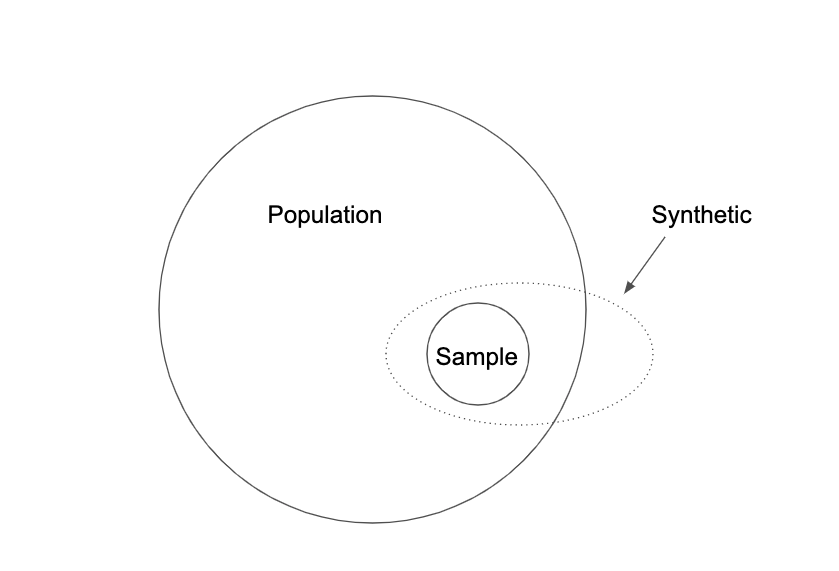
\includegraphics[width=0.75\linewidth]{../analysis/relationship.png}
	\caption{Relationship between population, sample and synthetic data \cite{Li.2006}}
	\label{fig:relationship}
\end{figure}

The next sections will describe an effective way to tackle the small dataset
problem. In chapter 2, the previously studied solutions are reviewed. A detailed
description of the proposed method is presented in chapter 3. This is followed
by the research methodology and the experimental results in chapters 4 and 5.
Finally, the paper is concluded with an analysis of the experimental results in
chapter 6.

\section{Related work}

Several data pre-processing methods to increase the data size have been
presented by the research community. In this section, the most important
approaches are reviewed and the state-of-the-art to improve small dataset
learning is reported. We start by describing fuzzy theories, which have
historically been the most used approach to mitigate the small dataset problem.
Next, we look at re-sampling mechanisms, which mainly consist of bootstrapping
techniques, and finally, we review over-sampling methods that can be a valuable
option to increase the sample size in small datasets.

\subsection{Fuzzy theories}

Many artificial sample generation techniques presented in the literature are
based on fuzzy theories \cite{AbdulLateh.2017}. The fuzzy set theory provides a
strict mathematical framework to generalize the classical notion of a dataset.
It gives a wider scope of applicability, especially in the fields of information
processing and pattern classification \cite{Zimmermann.2010}. Based on this
concept, several methods have emerged in the last decade to estimate or
approximate functions which are generating artificial samples for sparse
training sets. Figure \ref{fig:small-data-distribution} presents the obtained
samples and information gaps on the distribution of a small dataset.

\begin{figure}[H]
	\centering
	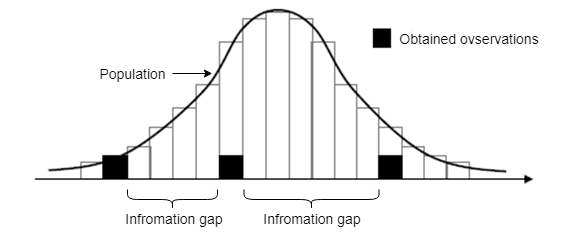
\includegraphics[width=0.6\linewidth]{../analysis/small_data_distribution.png}
	\caption{Distribution of a small dataset \cite{Tsai.2015}}
	\label{fig:small-data-distribution}
\end{figure}

The fundamental concept of creating synthetic data is called Virtual Sample
Generation (VSG) and was originally proposed by \cite{Niyogi.1998}. The idea is
to create additional observations based on the current set of examples by using
prior information. The introduction of virtual examples expands the effective
training set size and can therefore help to mitigate the learning problem.
\cite{Niyogi.1998} showed that the process of creating artificial samples is
mathematically equivalent to incorporating prior knowledge. They demonstrated
the concept on object recognition by mathematically transforming the views of
3D-objects. These new views are called virtual samples and its application
extends information and results in successful generalization of the proposed
solution.

Based on the above approach, several closely related studies were developed for
manufacturing environments. The first method to overcome scheduling problems due
to the lack of data in early stages of manufacturing systems was the creation of
a Functional Virtual Population (FVP) \cite{Li.2003}. The idea was to create a
number of virtual samples within a newly defined domain range. The method
involves a highly manual process, however, the application of FVP dramatically
improved the classification accuracy of a neural network. 

In 2004, the idea of fuzzifying information to extend a small dataset was used
to develop the Diffusion-Neural-Network (DNN) method \cite{Huang.2004}. It
combines the principle of information diffusion by \cite{Huang.1997} with
traditional Neural Networks to estimate functions. The information diffusion
method partially fills the information gaps by using fuzzy theories to represent
the similarities between samples and subsequently derive new ones. 

In order to fully fill the information gaps, a technique which diffuses the
sample set one for one was introduced by \cite{Li.2007}. Their concept is to
combine data trend estimation with a diffusion technique to estimate the domain
range mainly to avoid over-estimation. The method is called Mega-Trend-Diffusion
(MTD) and diffuses a set of data instead of each sample individually. For
example, the two samples $\mathit{m}$ and $\mathit{n}$ of figure
\ref{fig:mtd-function} are diffused simultaneously into one function with their
borders $\mathit{a}$ and $\mathit{b}$. To estimate $\mathit{a}$ and
$\mathit{b}$, the algorithm takes the minimum and maximum values of the dataset
and counts the number of data points which are smaller or greater than the
average of the values. This takes the skewness in the distribution of the data
and the domain range into consideration when calculating new samples. The
triangular shape of \ref{fig:mtd-function} represents the membership function
which shows the similarities between samples. $\mathit{M}$ and $\mathit{n}$ are
the samples and their heights are the possible values of the membership
function.

\begin{figure}[H]
	\centering
	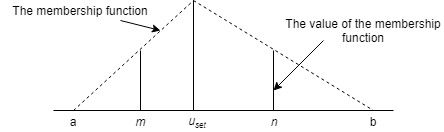
\includegraphics[width=0.6\linewidth]{../analysis/mtd_function.png}
	\caption{MTD function \cite{Li.2007}}
	\label{fig:mtd-function}
\end{figure}

After estimating the domain range between $\mathit{a}$ and $\mathit{b}$, samples
are randomly produced within this area by using a common diffusion function. The
artificial samples are then trained with a Back-propagation Neural Network
(BPNN) like \cite{Huang.2004} originally proposed. This technique is seen as an
improvement of DNN and was initially developed to improve early flexible
manufacturing system scheduling accuracy. In further research, MTD is widely
used as a synthetic sample generation method and is recognized as an effective
way to deal with small dataset problems \cite{AbdulLateh.2017}. However, MTD
only considers the data for independent attributes and does not deal with their
relationships. 

Also, a genetic algorithm based virtual sample generation (GABVSG) was proposed.
The method takes the relationship among the attributes into account and explores
the integrated effects of attributes instead of dealing with them individually.
This algorithm is performed in three steps: Samples are randomly selected to
determine the range of each attribute by using MTD functions. Next, a Genetic
Algorithm is applied to find the most feasible virtual samples. Finally, the
average error of these new samples is calculated. The results outperformed the
ones using MTD and also showed better performance in prediction than in case of
no generation of synthetic samples \cite{Li.2014}.

\subsection{Random over-sampling}

An alternative approach to fuzzy theories as well the most well-known artificial
sample generation method is the Bootstrapping Procedure (BP)
\cite{AbdulLateh.2017} or Random Over-Sampling (ROS) as is known in the
imbalanced learning research area. The main difference to the previously
presented techniques is that ROS creates expands the training set by resampling
instances from the measured data with replacement \cite{Efron.1993}. Therefore,
it allows the algorithms to use the same sample more than one time to gradually
revise the identified patterns in order to improve predictive accuracy. However,
ROS may cause over-fitting when applied to small data because it repetitively
uses the same information \cite{Tsai.2015}, \cite{Li.2018}. Nevertheless,
\cite{Ivanescu.2006} applied ROS in batch process industries where it was shown
that it may help mitigate the limited data problem.

\subsection{Informed over-sampling}

A different approach to fill information gaps is informed over-sampling. It is
an artificial data generation strategy originally developed in the context of
machine learning to mitigate the imbalanced learning problem. Its origin comes
from a different research community than the fuzzy strategies presented above,
which is more related to machine learning techniques. Although over-sampling,
fuzzy theories and bootstrapping approaches are aiming to solve a similar
problem, it seems that these communities have had very few connections so far.

In the imbalanced learning problem, the classes of the given dataset are
significantly skewed i.e. the dataset has a large number of observations in one
of the classes called majority class and relatively small number of observations
in the other class(es) called minority class(es). This constitutes a problem for
the learning phase of the algorithm resulting in low accuracy for the minority
class(es). In practice, the imbalanced dataset problem is very common issue in
supervised learning. Especially, in the fields of fraud detection, product
categorization and disease diagnosis, an imbalanced dataset is the norm rather
than the exception \cite{He.2013}. 

\subsubsection{SMOTE}

There are several methods presented in the literature that belong in the
over-sampling category. The first method to be  proposed and still the most
popular is the Synthetic Minority Oversampling TEchnique (SMOTE). SMOTE is based
on the idea of k-nearest neighbors and linear interpolation as a data generation
mechanism. More specifically, SMOTE proposes to form a line segment between
neighboring minority class instances and generate synthetic data between them
\cite{Chawla.2002}. The algorithm is very popular due to its simplicity as well
as its robustness. Numerous variations have been proposed based on SMOTE,
increasing its status as the staple idea in over-sampling for imbalanced
learning problems \cite{Fernandez.2018}. However, SMOTE has some significant
limitations when it comes to the sample generation process. In practice, the
separation between majority and minority class areas is often not clearly
definable. Thus, noisy samples may be generated when a minority sample lies in
the region of the majority classes. Figure \ref{fig:noisy-examples} presents a
scenario where a minority instance is generated within the majority region
(noisy sample).

\begin{figure}[H]
	\centering
	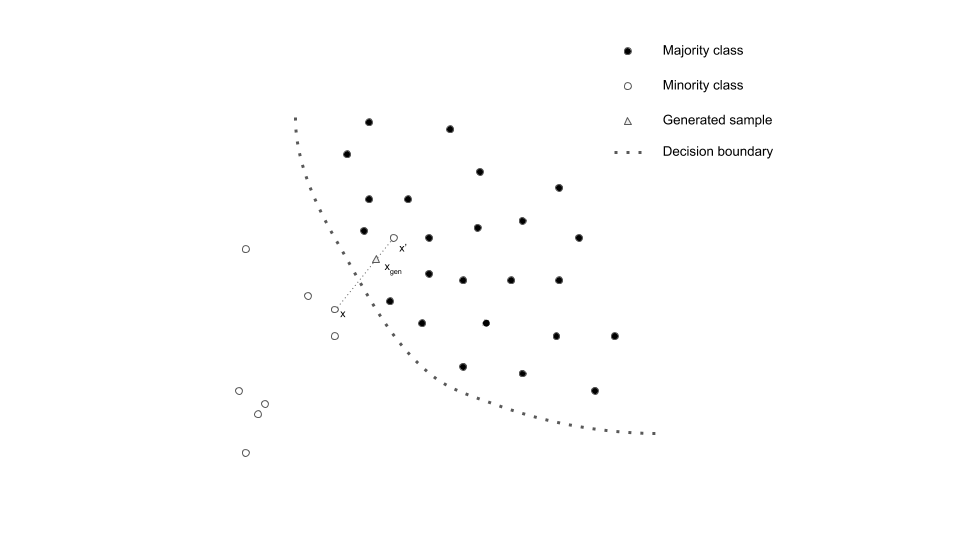
\includegraphics[width=0.6\linewidth]{../analysis/noisy_examples.png}
	\caption{Generation of noisy examples \cite{Douzas.2019b}}
	\label{fig:noisy-examples}
\end{figure}

Furthermore, redundant instances may be generated within dense minority regions,
as so that they do not add any relevant information to the classifier and may
lead to over-fitting. Figure \ref{fig:redundant-examples} demonstrates an
example where a minority  class instance is generated in a dense minority class.
This new observation belongs to the same dense cluster as the original and is
therefore less useful. 

\begin{figure}[H]
	\centering
	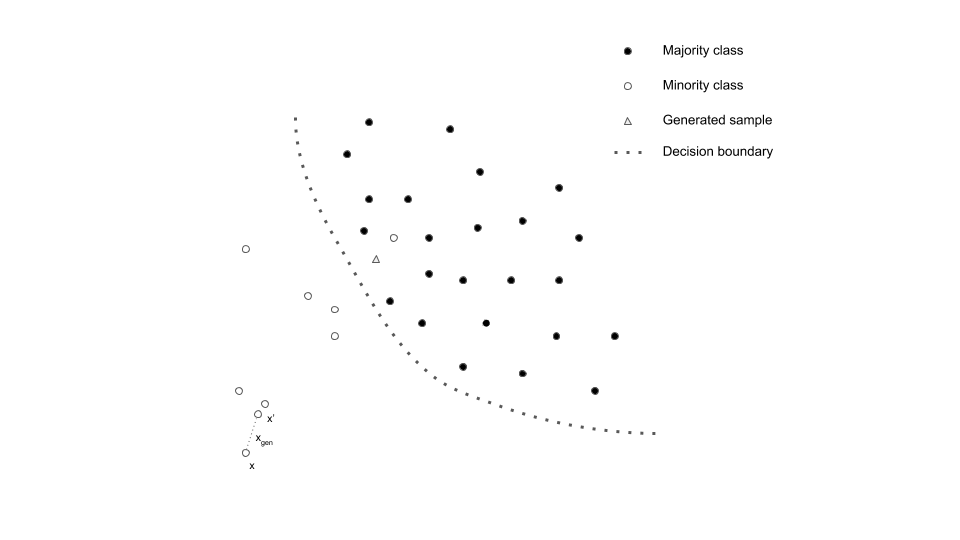
\includegraphics[width=0.6\linewidth]{../analysis/redundant_examples.png}
	\caption{Generation of redundant examples \cite{Douzas.2019b}}
	\label{fig:redundant-examples}
\end{figure}

Although SMOTE is recognized as an over-sampling technique for imbalanced
datasets, it can also be used for solving the small dataset problem.
\cite{Li.2018} showed that SMOTE is able to successfully fill the information
gaps with synthetic samples. However, given its limitations, SMOTE did not
achieve the best results within their study.

\subsubsection{G-SMOTE}

The novel data generation procedure Geometric SMOTE (G-SMOTE) has been presented
with the objective to improve the above mentioned limitations of the SMOTE
algorithm \cite{Douzas.2019b}. G-SMOTE can be seen as a substitute of SMOTE
enhanced by geometric properties. The main difference to SMOTE is that it
broadens the options for data generation and prevents the creation of noise.
Instead of connecting a minority sample and one of its minority class nearest
neighbors with a line segment, the instances are generated in a geometrical
region around the minority sample. Furthermore, G-SMOTE is designed to avoid the
generation of noisy samples by introducing the \textit{selection strategy}
hyper-parameter. Figure \ref{fig:smotevsgsmote} demonstrates the distribution of
artificially created samples by SMOTE versus G-SMOTE. Increasing number of
$\mathit{k}$ neighbors, SMOTE tends to generate noisy samples, whereas G-SMOTE
avoids this scenario.

\begin{figure}[H]
	\centering
	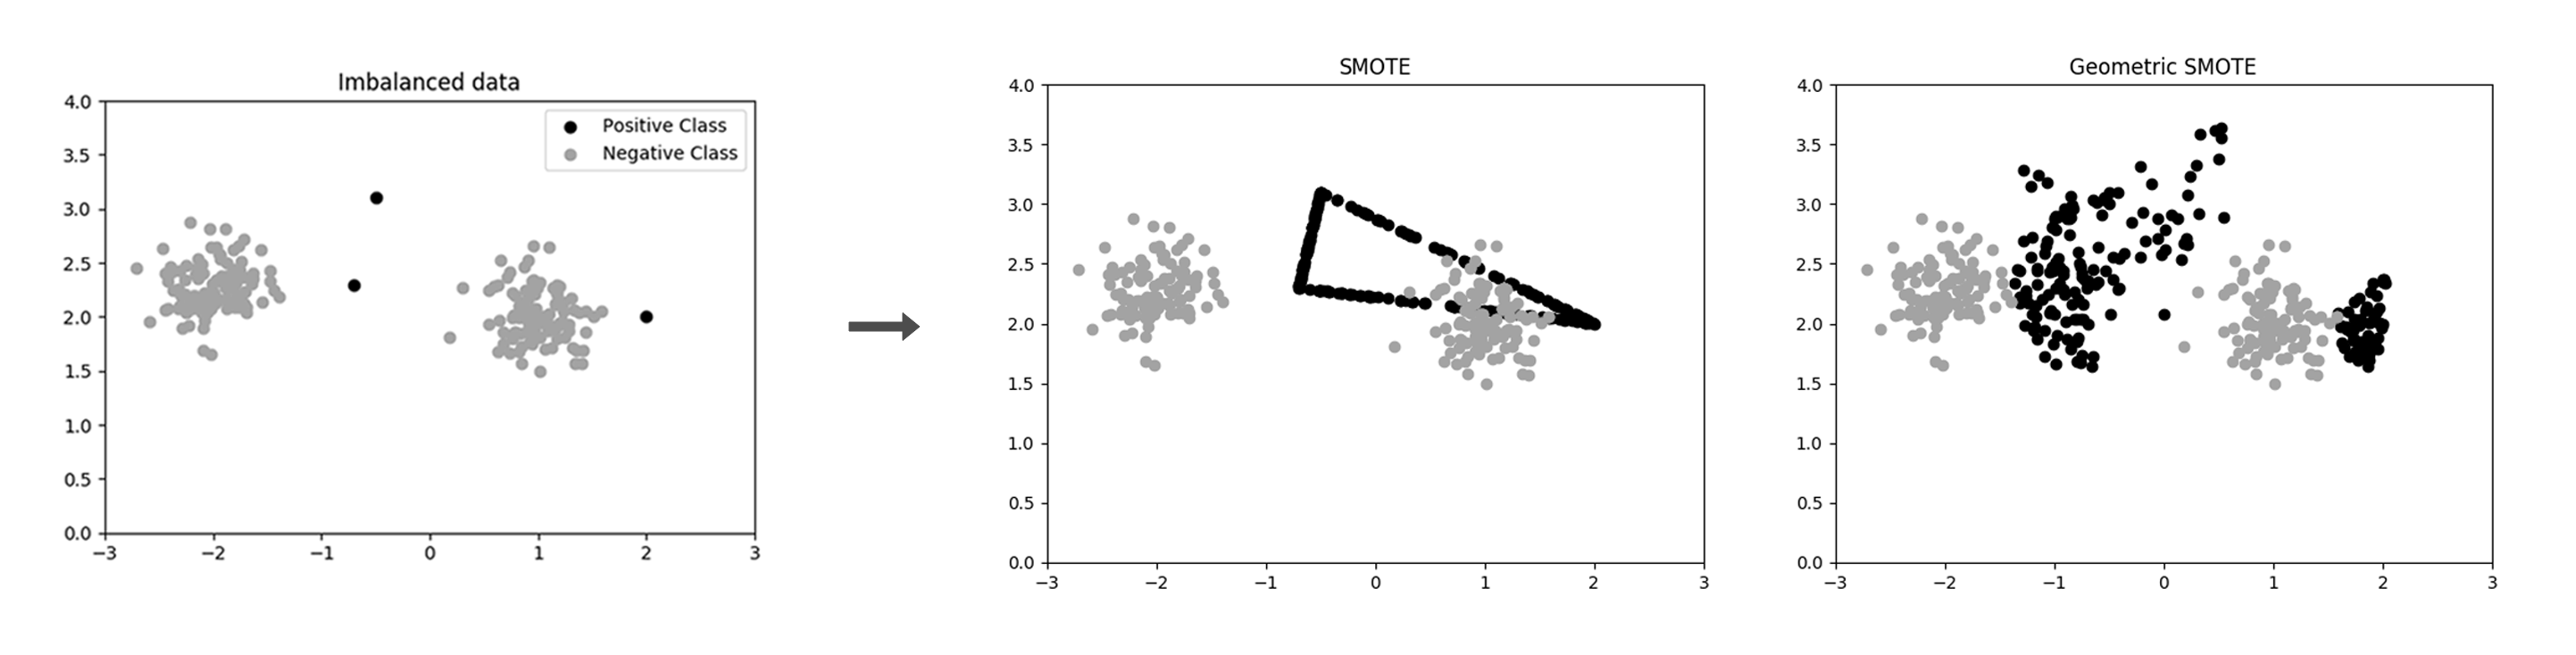
\includegraphics[width=1\linewidth]{../analysis/smote_vs_gsmote}
	\caption{SMOTE versus G-SMOTE \cite{Douzas.2019}}
	\label{fig:smotevsgsmote}
\end{figure}

The study of \cite{Douzas.2019b} has performed an extensive comparison between
G-SMOTE and SMOTE using 69 imbalanced datasets and several classifiers. The
results show that G-SMOTE outperforms SMOTE, Random Oversampling and the case of
no over-sampling, across all datasets, classifiers and performance metrics.

\section{Proposed method}

In the following section, we present G-SMOTE as a novel data generation
procedure for small datasets in the case of binary classification. Originally
developed for the imbalanced learning problem, we adapt the algorithm to not
only re-sample the minority class, but the entire dataset independent from the
class distribution. 

\subsection{G-SMOTE for the small dataset problem}

As mentioned above, the G-SMOTE algorithm randomly generates artificial data
within a geometrical region of the input space. The size of this area is derived
from the distance of the selected sample to one of its nearest neighbors,
whereas the shape is determined by the hyper-parameters called
\textit{truncation factor} and \textit{deformation factor}. Additionally, the
\textit{selection strategy} hyper-parameter  of G-SMOTE modifies the standard
SMOTE selection process and also affects the size of the geometric region.
Although the main concept can be adapted from the original method to the small
dataset problem, the \textit{selection strategy} requires some minor adjustments which
will be described hereafter. In what follows, G-SMOTE is applied to the case of
binary classification tasks. The application for the multi-class case is also
straightforward and it is based on the binarization of the problem through the
one-vs-all approach. Finally, regression tasks require an extensive modification
of the original G-SMOTE algorithm and they will be a topic of future research.

The \textit{selection strategy} hyper-parameter \( \alpha_{sel} \) defines the
radius of the geometric region. This mechanism allows the positive or negative
class area to expand into the feature space but at the same time prevents the
algorithm from creating noisy samples. In G-SMOTE for small data both classes
are selected in two individual runs to introduce new observations. In the first
run, a random sample called \( \textbf{x}_{surface} \) is selected which belongs
to the positive class. Similarly, \( \textbf{x}_{surface} \) is assigned to the
negative class samples in the second run. Both runs are based on the defined
selection strategy where \( \alpha_{sel} \) can have three different values:
positive class selection \( S_{pos} \), negative class selection \( S_{neg} \)
and combined selection \( S_{com} \). We describe the cases referring to first
run of randomly selecting a positive sample. In the second run, a negative class
example is randomly chosen and the process is repeated inversely. 

\begin{enumerate}[label=($\alph*$)]

\item Positive class selection

With the hyper-parameter selection\_strategy = 'positive', a second positive 
class sample is selected as one of the \( k \) nearest neighbors. This 
indicates that the selection strategy is based only on the positive class and 
works like the selection strategy of SMOTE. As SMOTE may lead to the generation 
of data penetrating the opposite class area, this drawback also applies on the 
selection strategy here.

\begin{figure}[H]
	\centering
	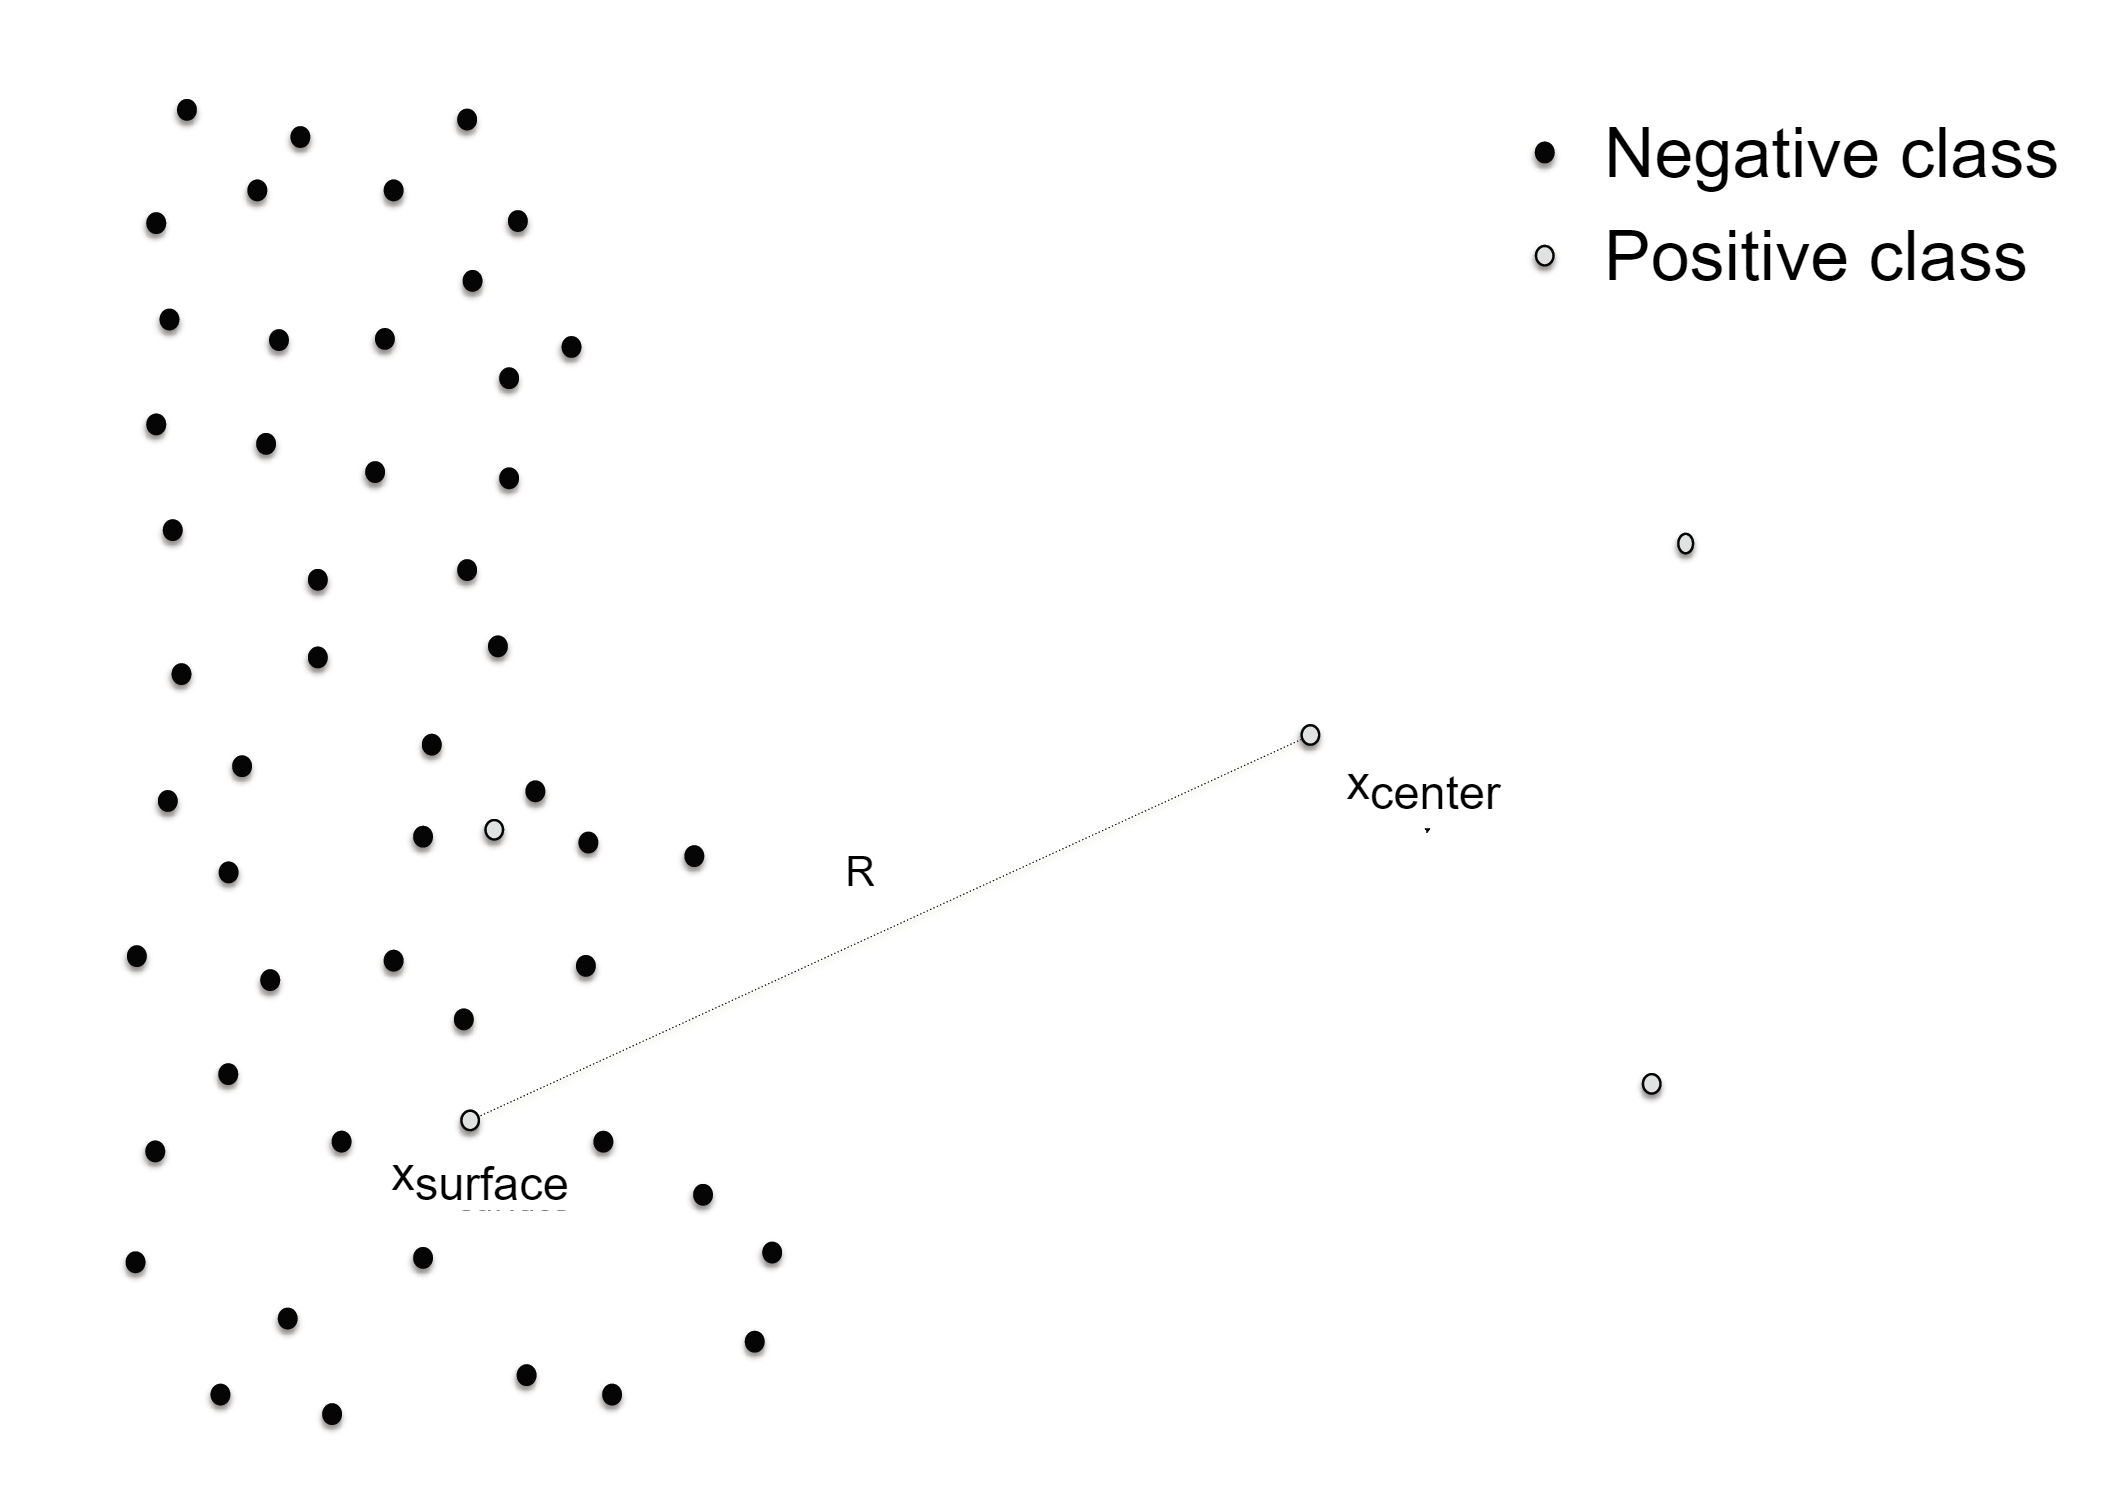
\includegraphics[width=0.51\linewidth]
		{../analysis/positive_class_selection_strategy}
	\caption{Example of positive class selection strategy: A positive class 
	instance is defined as the center and one of its \( k = 4 \) positive 
	class nearest neighbors is selected as the surface point. The radius 
	\( R \) is equal to the distance of these instances 
	\cite{Douzas.2019b}.}
	\label{fig:positiveclassselectionstrategy}
\end{figure}

\item Negative class selection

When selection\_strategy = 'negative', a negative sample is selected as the 
nearest class neighbor. This scenario prevents the algorithm from creating 
noisy samples. More specifically, as the radius is drawn from the selected 
positive class instance to the nearest neighbor of the negative class, it does 
not allow the data generation mechanism to penetrate the opposite area.

\begin{figure}[H]
	\centering
	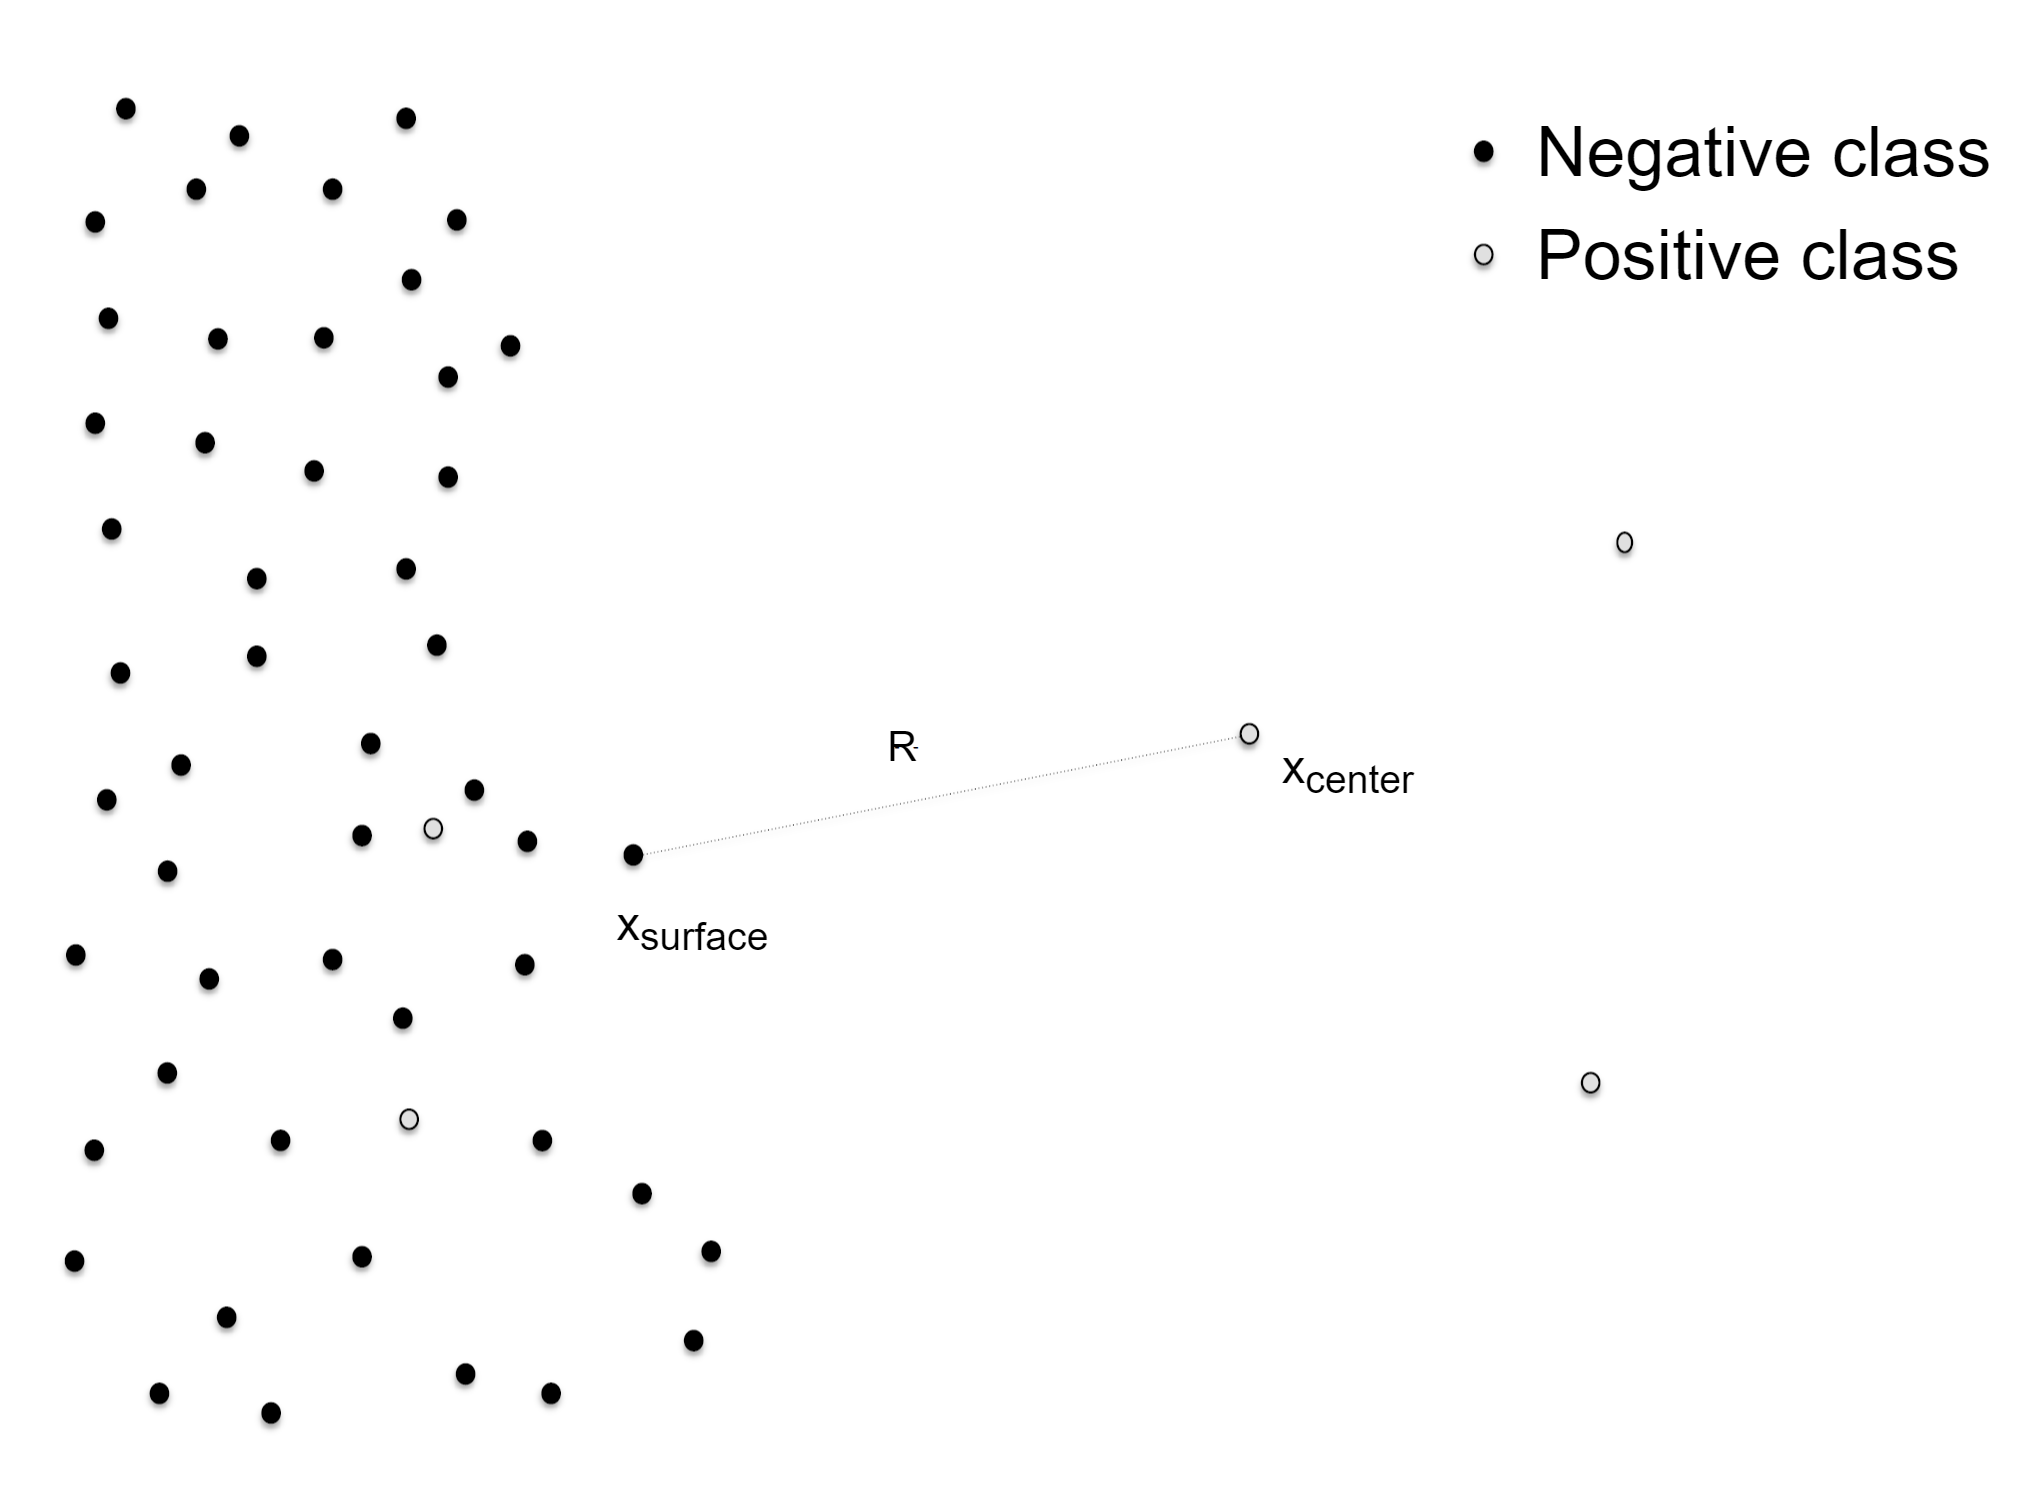
\includegraphics[width=0.5\linewidth]
		{../analysis/negative_class_selection_strategy}
	\caption{Example of negative class selection strategy: A positive class 
	instance is defined as the center and its closest negative class neighbor 
	is selected as the surface point. The radius \( R \) is defined to be 
	equal to the distance of these instances \cite{Douzas.2019b}.}
	\label{fig:negativeclassselectionstrategy}
\end{figure}

\item Combined selection

The combined selection strategy initially applies the positive and negative 
selection strategies. Once \( \textbf{x}_{pos} \) and \( \textbf{x}_{neg} \) 
are identified, the point with the minimum distance to the center \( 
\textbf{x}_{center} \) is defined as the surface point \( \textbf{x}_{surface} 
\). Figure 10 presents an example when \( \textbf{x}_{surface} \) is identified 
as a negative class instance.

\begin{figure}[H]
	\centering
	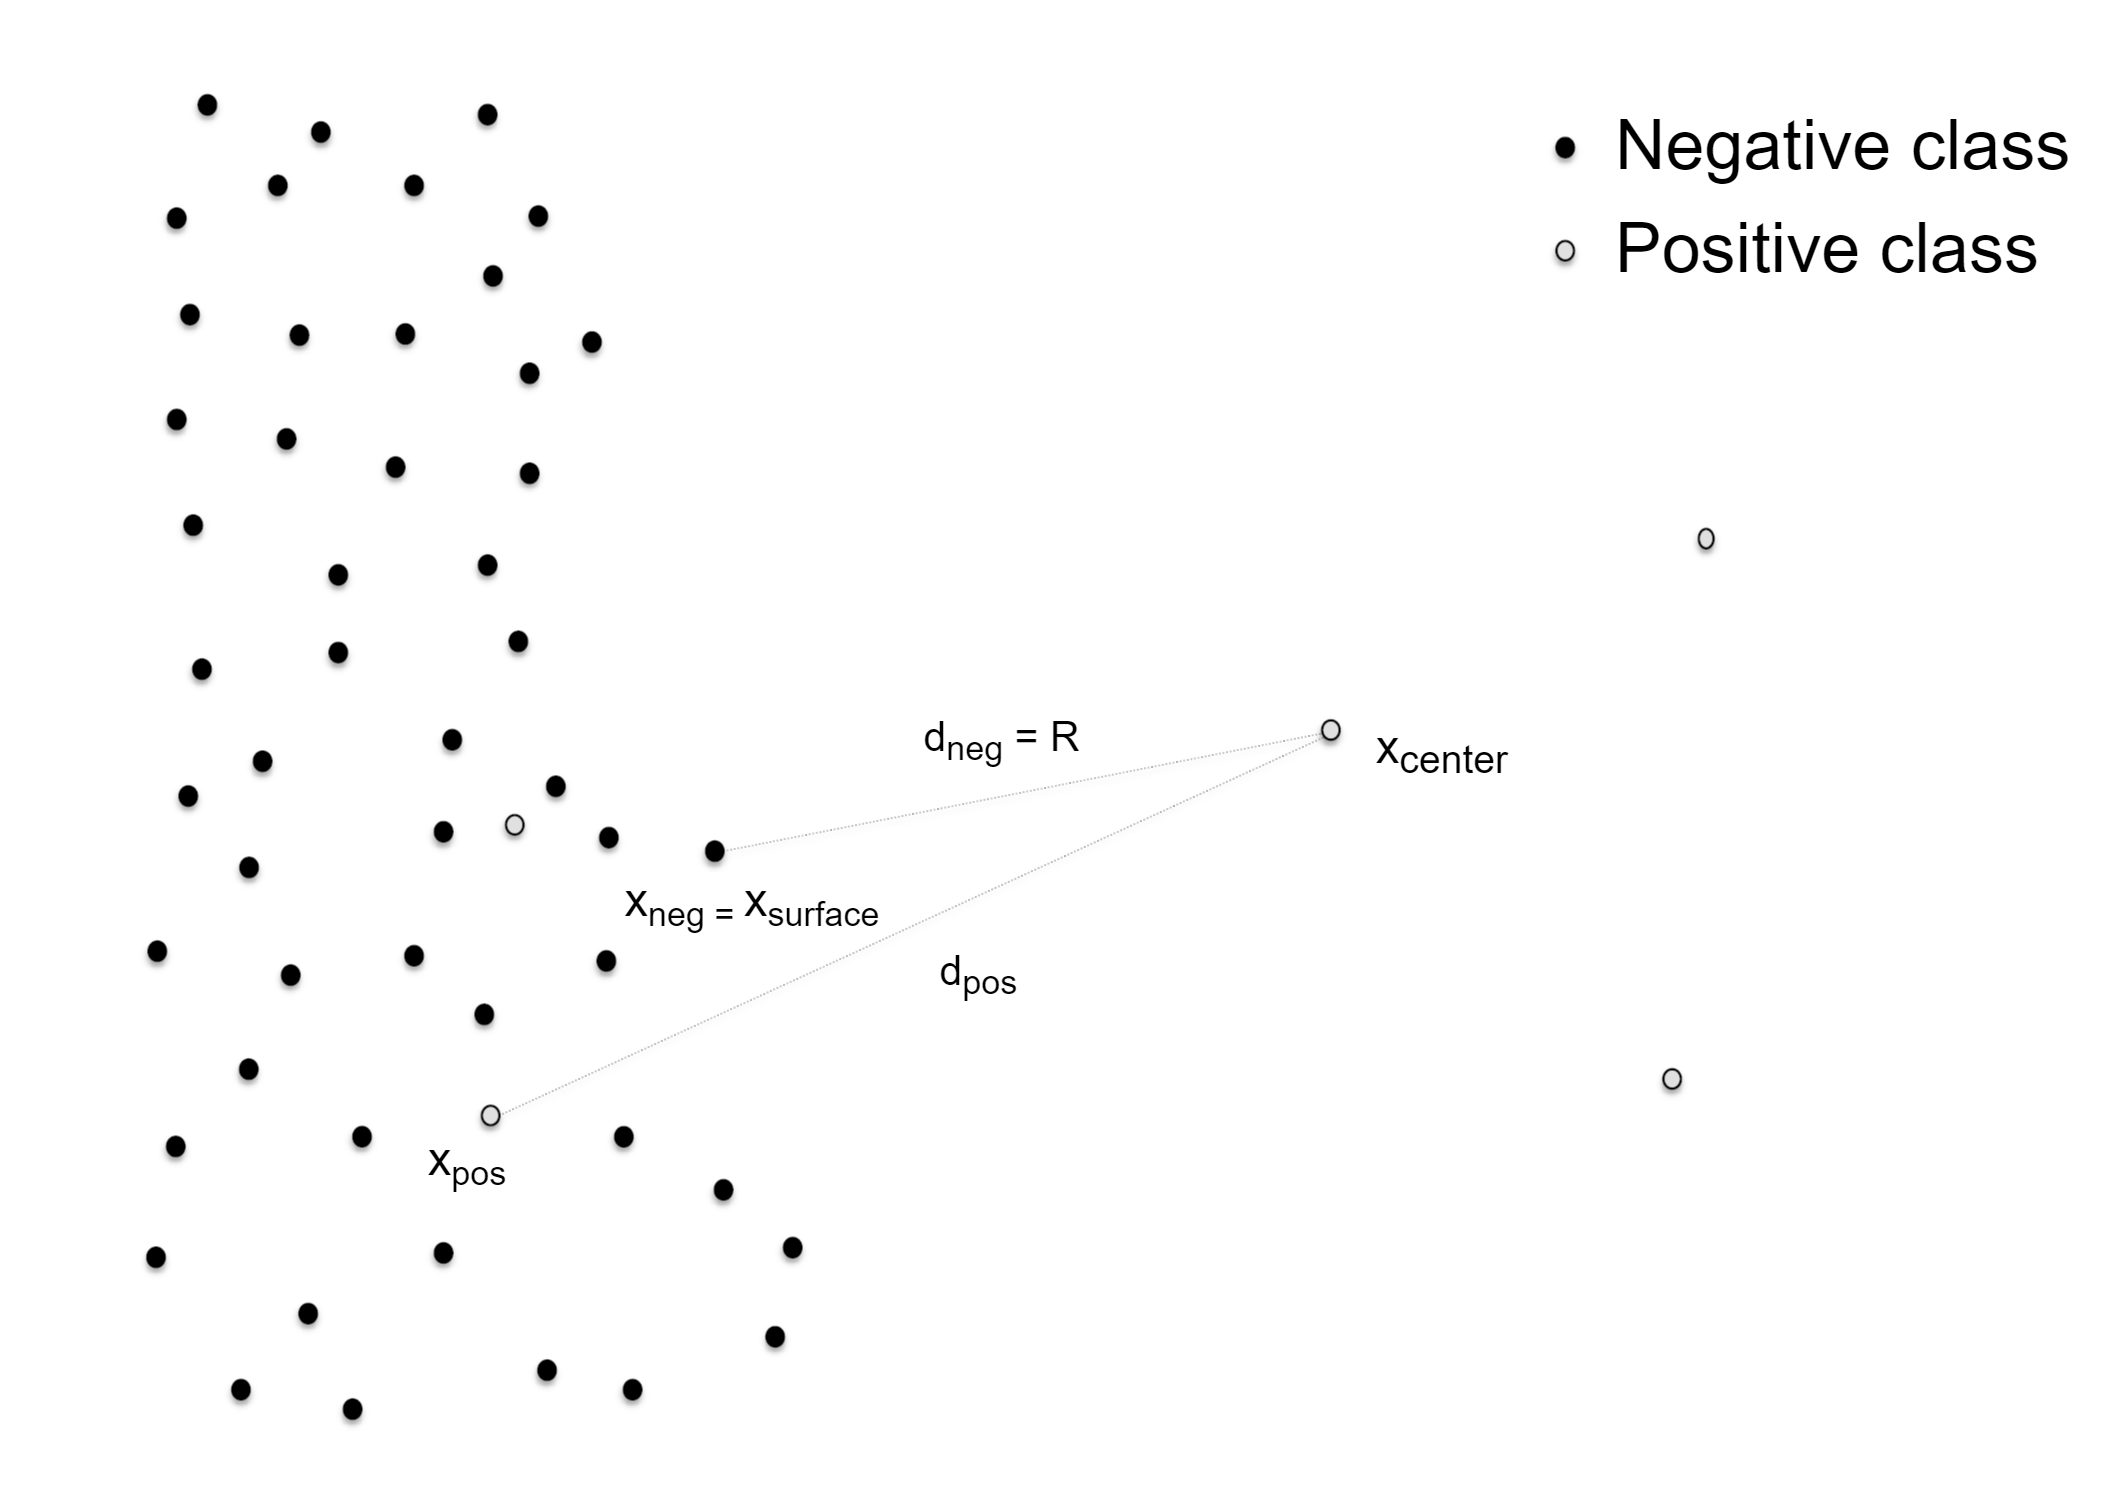
\includegraphics[width=0.52\linewidth]
		{../analysis/combined_class_selection_strategy}
	\caption{The closest point \( \textbf{x}_{neg} \) to the center positive 
	class sample \( \textbf{x}_{center} \) is identified as the surface point 
	\( \textbf{x}_{surface} \) since it is closer to the center than the 
	selected instance \( \textbf{x}_{pos} \) from the \( k \) nearest 
	positive class neighbors of the center \cite{Douzas.2019b}.}
	\label{fig:combinedclassselectionstrategy}
\end{figure}

\end{enumerate}

\subsection{Adapted G-SMOTE algorithm}

The adapted G-SMOTE algorithm can be generally described in the following steps:

\begin{enumerate}
	\item 
	An empty set \( S_{gen} \) is initialized
	\item 
	The \( S_{pos} \) elements are shuffled and the process described 
	below is repeated \( N \) times until \( N \) artificial points 
	have been generated.
	\item 
	A positive class instance \( \textbf{x}_{center} \) is selected as the 
	center of the geometric region.
	\item 
	Depending on the values of \( \alpha_{sel} \) (positive, negative 
	or both), this step results in a randomly selected sample 
	\( \textbf{x}_{surface} \) which belongs either to the positive or negative 
	sample set
	\item 
	A random point \( \textbf{e}_{sphere} \) is generated on the surface of a 
	unit hypersphere centered at the origin of the input space. This point is 
	transformed to a randomly generated point \( \textbf{x}_{gen} \) inside the 
	unit hypersphere. 
	\item 
	The geometrical transformations are applied to define the admissible area 
	for \( \textbf{x}_{gen} \). These are defined as truncation 
	\( \alpha_{trunc} \), which defines the subarea of the hypersphere 
	and deform \( \alpha_{def} \), which deforms the hypersphere. 
	
	\begin{enumerate}[label=($\alph*$)]
		\item 
		The truncation factor \( \alpha_{trunc} \) defines the degree 
		of truncation that is applied to the geometric area and can be 
		specified between zero and one, where truncation factor = 0.0 
		corresponds to a circle and truncation factor = 1.0 becomes a 
		half-hypersphere around the selected sample. 
		
		\item 
		The formation of the area is defined by the so-called deformation 
		factor. If the parameter of the deformation factor is equal to 0, the 
		data generation area obtains a circle. On the opposite, if the 
		parameter is set to 1, the area deforms to a line segment. 
		For a graphical example of these hyper-parameters the reader is 
		referred to (Douzas, 2019).
	\end{enumerate}

	\item 
	The generated point \( \textbf{x}_{gen} \) is translated
	\item 
	\( \textbf{x}_{gen} \) is added to \( \textbf{S}_{gen} \)
	\item 
	Once this process is repeated \( N \) times: \( \textbf{x}_{neg} \) 
	elements are shuffled, a negative class instance is selected as 
	\( \textbf{x}_{center} \) and the algorithm starts again with step 4 until 
	\( N \) negative samples are introduced
\end{enumerate}

\section{Research methodology}

The main objective of this work is to compare G-SMOTE with other oversampling
techniques when it comes to the small dataset problem. Therefore, we use a
variety of datasets, evaluation measures and classifiers to evaluate the
performance. A description of this set-up, the experimental procedure as well as
the software implementation is provided in this section.

\subsection{Experimental data}

Ten datasets are used to test the performance of G-SMOTE which are retrieved
from UCI Machine Learning Repository \cite{Dua.2019}. The focus on the selection
of the data lies on binary classification problems with a highly balanced
distribution of the two classes. In order to assure generalizability of the
results, the datasets include different topics such as health care, finance,
business and physics as well as different sample sizes. Details of the datasets
are presented in the following table:

\begin{longtable}{llll}
	\specialrule{.1em}{.05em}{.05em}
	\textbf{Dataset} & \textbf{Number of samples} & \textbf{Number of
	attributes} & \textbf{Area} \\
	\hline
	Arcene & 900 & 10.000 & Health Care \\
	Audit & 776 & 18 & Business \\
	Banknote Authentication & 1.372 & 5 & Finance \\
	Spambase & 4.610 & 57 & Business\\
	Breast Cancer & 699 & 10 & Health Care\\
	Indian Liver Patient & 583 & 10 & Health Care\\
	Ionosphere & 351 & 34 & Physics\\
	MAGIC Gamma Telescope & 19.020 & 11 & Physics\\
	Musk & 6.598 & 168 & Physics\\
	Parkinsons & 197 & 23 & Health Care\\
	\specialrule{.1em}{.05em}{.05em}
\caption{\label{tab:datasets}Description of the datasets} 
\end{longtable}

\subsection{Evaluation measures}

To evaluate the performance of G-SMOTE, the experiment includes two different
measures. First, accuracy is used as one of the most common metrics for
evaluating classification models \cite{M.2015}. Accuracy measures the ratio of
correct predictions over the total number of instances evaluated. The accuracy
metric can be stated as

$$Accuracy = \frac{TP + TN}{TP +TN + FP + FN}$$

where \( TP \), \( TN \) denote the number of correctly classified positive as
well as negative instances and \(FP \), \( FN\) denote the number of
misclassified negative and positive instances, respectively. The accuracy metric
might be inappropriate for datasets with a significant difference between the
number of positive and negative classes. As pointed out by many studies,
accuracy has limitations in the discrimination process since rare classes have
only few impacts on the measure compared to majority classes. To make sure the
contribution in the accuracies of the two classes stay relatively balanced, we
include the geometric mean score (G-Mean) as a second measure. G-Mean measures
the trade-off between sensitivity (true positive rate) and specificity (true
negative rate) by the following:

$$G-Mean = \sqrt{sensitivity \times specificity} = \sqrt{\dfrac{TP}{TP + FN} 
\times \dfrac{TN}{TN + FP}}$$

\subsection{Machine learning algorithms}

The experiment is conducted with several classifiers to make sure the results
are not dependent on the machine learning algorithm. We use the following four
classifiers: Logistic Regression (LR) \cite{McCullagh.2019}, K-Nearest Neighbors
(KNN) \cite{Cover.1967}, Decision Tree (DT) \cite{Salzberg.1994} and Gradient
Boosting (GB) \cite{Friedman.2001}.

\subsection{Experimental procedure}

The main concept of the experimental procedure is to randomly under-sample the
datasets presented in table \ref{tab:datasets}, increase their size artificially with
different over-samplers and compare the results with the original dataset which
is considered to be the benchmark. This method allows us to directly compare the
quality of the artificial generated sample set with the observed data. In order
to evaluate if the proposed method can improve artificial data generation, we
compare G-SMOTE with SMOTE, Borderline SMOTE and Random Oversampling. Also, we
apply the machine learning algorithms to the under-sampled data with the
objective to assess their performance with a smaller amount of data. To
under-sample the data we use a ratio of 50, 75, 90 and 95 percent of the
original dataset. For example, with an undersampling ratio of 95 percent, we
take only five percent of the original data as a base to apply the over-sampling
mechanism. This approach aims to provide an understanding of the classification
performance as the size of the dataset diminishes.

Figure \ref{fig:experimentalprocedure} visualizes the experimental process: 

\begin{figure}[H]
	\centering
	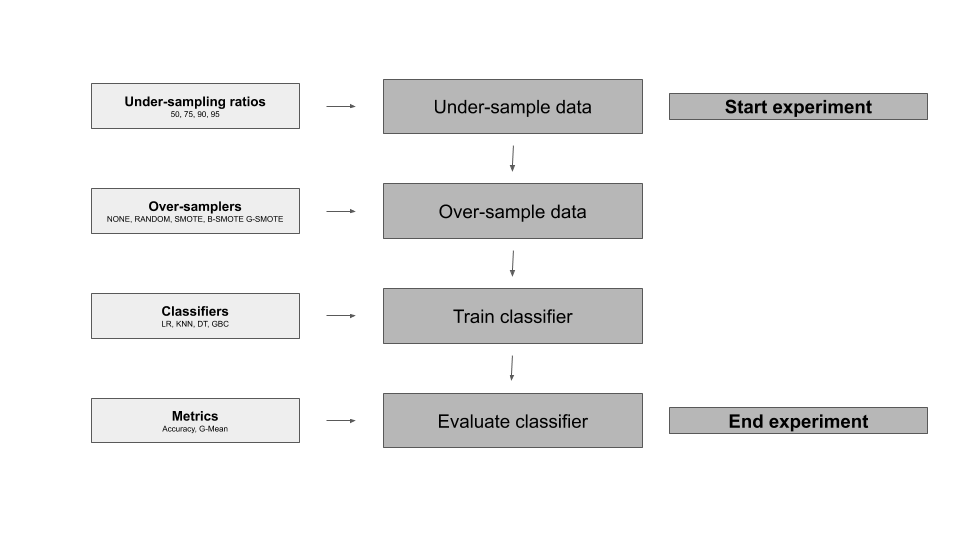
\includegraphics[width=0.7\linewidth]{../analysis/experimental_procedure.png}
	\caption{High-level experimental procedure}
	\label{fig:experimentalprocedure}
\end{figure}

We use \( k \)-fold cross-validation scores with \( k = 5 \) to assess the
performance of the models for each combination of over-sampler and classifier.
The dataset \( D \) is randomly split into \( k \) subsets (folds) \( D_1, D_2,
… D_k \) of approximately equal size. Each fold is used as a validation set and
the remaining folds are used to train the model with \( k \) iterations. This
procedure is repeated until each \( k \) have been used as a validation set
\cite{Han.2012}. Based on the above description, the experiment is conducted in
the following steps within one iteration:

\begin{enumerate}
	
	\item 
	Splitting dataset into \( k \)-fold cross-validation sets where \( k \).

	\item 
	Undersampling \( k - 1 \) folds such that the class frequency remains 
	the same as the original with a ratio of 50, 75, 90 and 95 percent.

	\item 
	Synthetic oversampling of \( k - 1 \) folds to the original size of the
	dataset (class ratio remains the same) with G-SMOTE, SMOTE, Borderline
	SMOTE, Random Oversampling and No Oversampling.

	\item 
	Training the model with the classifiers LR, KNN, DT and GB

	\item 
	Testing the model with the remaining, original fold

	\item 
	Computation of results

\end{enumerate}	

This procedure is repeated 3 times and the highest cross validation score for
each combination of dataset, classifier, oversampler and evaluation metric is
reported.

In order to confirm the statistical significance of the experimental results,
the Friedman test \cite{Sheldon.1996} as well as the Holm test
\cite{JanezDemsar.2006} are applied. Ranking scores are assigned to each
over-sampling method with scores of 1 to 5 for the best and worst performing
methods, respectively. The Friedman test is a non-parametric procedure that
compares the average rankings of the algorithms under the null hypothesis that
all show identical performance independent of the selected classifier and
evaluation metric. If the null-hypothesis is rejected to our favor, we proceed
with the Holm test. The Holm test acts as a post-hoc test for the Friedman test
for controlling the family-wise error rate when all algorithms are compared to a
control method and not between themselves. This non-parametric test is very
powerful in situations where we want to test whether a newly proposed method is
better than existing ones. The control method in our case is the proposed
G-SMOTE method and is tested under the null hypothesis that it performs
similarly to the rest of over-samplers for every combination of classifier and
metric.

\subsection{Software Implementation}

The implementation of the experimental procedure is based on Python programming
language using the Scikit-Learn library
\cite{PedregosaF.VaroquauxG.GramfortA.MichelV.ThirionB.GriselO.BlondelM.Prette.2011}.
All functions, algorithms, experiments and results reported are provided at
\url{https://github.com/AlgoWit/publications/tree/master/small-data-oversampling}.
Additionally, Research-Learn library
(\url{https://github.com/AlgoWit/research-learn}) provides a framework to
implement comparative experiments, being also fully integrated with the
Scikit-Learn ecosystem.

\section{Results and discussion}

In this section the performance of the different oversamplers and the results 
of the statistical tests are presented and analyzed.

\subsection{Comparative presentation}

The mean cross validation scores and the standard error per classifier and
metric across all datasets are presented in Table \ref{tab:mean_sem_scores}. The
scores are presented for each under-sampling ratio to evaluate how the methods
perform as the dataset size diminishes. We include the benchmark method that
represents the original dataset without applying under-sampling before training
the algorithm. This sample set is seen as the ground truth of our experiments
which is expected to obtain the best results by design.

\begin{center}
\begin{footnotesize}
\csvreader[
	longtable=lllllllll,
	table head=
	\toprule\mdseries Ratio & \mdseries Classifier & \mdseries Metric & \mdseries NONE & \mdseries 
	RANDOM & \mdseries SMOTE & \mdseries B-SMOTE & \mdseries G-SMOTE & \mdseries BENCHMARK \\
	\midrule\endhead
	\bottomrule\endfoot,
	late after line=\\,
	before reading={\catcode`\#12},
	after reading={\catcode`\#12},
	]{../analysis/mean_sem_scores.csv}
	{1=\ratio,2=\classifier,3=\metric,4=\none,5=\random,6=\smote,7=\bsmote,
		8=\gsmote,9=\benchmark}
	{\ratio & \classifier & \metric & \none & \random & \smote & \bsmote & 	
	\gsmote & \benchmark}
\end{footnotesize}
\addtocounter{table}{-1}
\captionof{table}{Results for mean cross validation 
	scores of oversamplers (NONE corresponds to No Oversampling, RANDOM 
	to Random Oversampling and B-SMOTE to Borderline SMOTE)}
\label{tab:mean_sem_scores}
\end{center}

This table shows that G-SMOTE outperforms nearly all over-sampling methods for
all combinations of classifiers and metrics. Throughout the scores we can
observe that all over-samplers have a better performance as the dataset increase
their size i.e. the under-sampling ratio gets smaller.  Particularly, the scores
of G-SMOTE are the closest to the ones of the Benchmark method which implies
that the proposed method is able to artificially establish a representative
dataset.

Table \ref{tab:mean_sem_perc_diff_scores} presents the mean and standard error
of percentage difference between G-SMOTE and No Oversampling. It shows that
G-SMOTE performs significantly better compared to the case where no
over-sampling is applied in every combination of under-sampling ratio,
classifier and metric. Particularly, the performance gap increases for higher
under-sampling ratios.

\begin{center}
	\begin{footnotesize}
		\csvreader[
		longtable=llll,
		table head=
		\toprule\mdseries Ratio & \mdseries Classifier & \mdseries Metric & \mdseries Difference \\
		\midrule\endhead
		\bottomrule\endfoot,
		late after line=\\,
		before reading={\catcode`\#12},
		after reading={\catcode`\#12},
		]{../analysis/mean_sem_perc_diff_scores.csv}
		{1=\ratio,2=\classifier,3=\metric,4=\difference}
		{\ratio & \classifier & \metric & \difference}
	\end{footnotesize}
	\addtocounter{table}{-1}
	\captionof{table}{Results for percentage difference between G-SMOTE and SMOTE}
	\label{tab:mean_sem_perc_diff_scores}
\end{center}

As explained in section 4, a ranking score in the range 1 to 5 is assigned to
each oversampler. The mean ranking of all oversampling methods across the
datasets is presented in the following figure: 

\begin{figure}[H]
	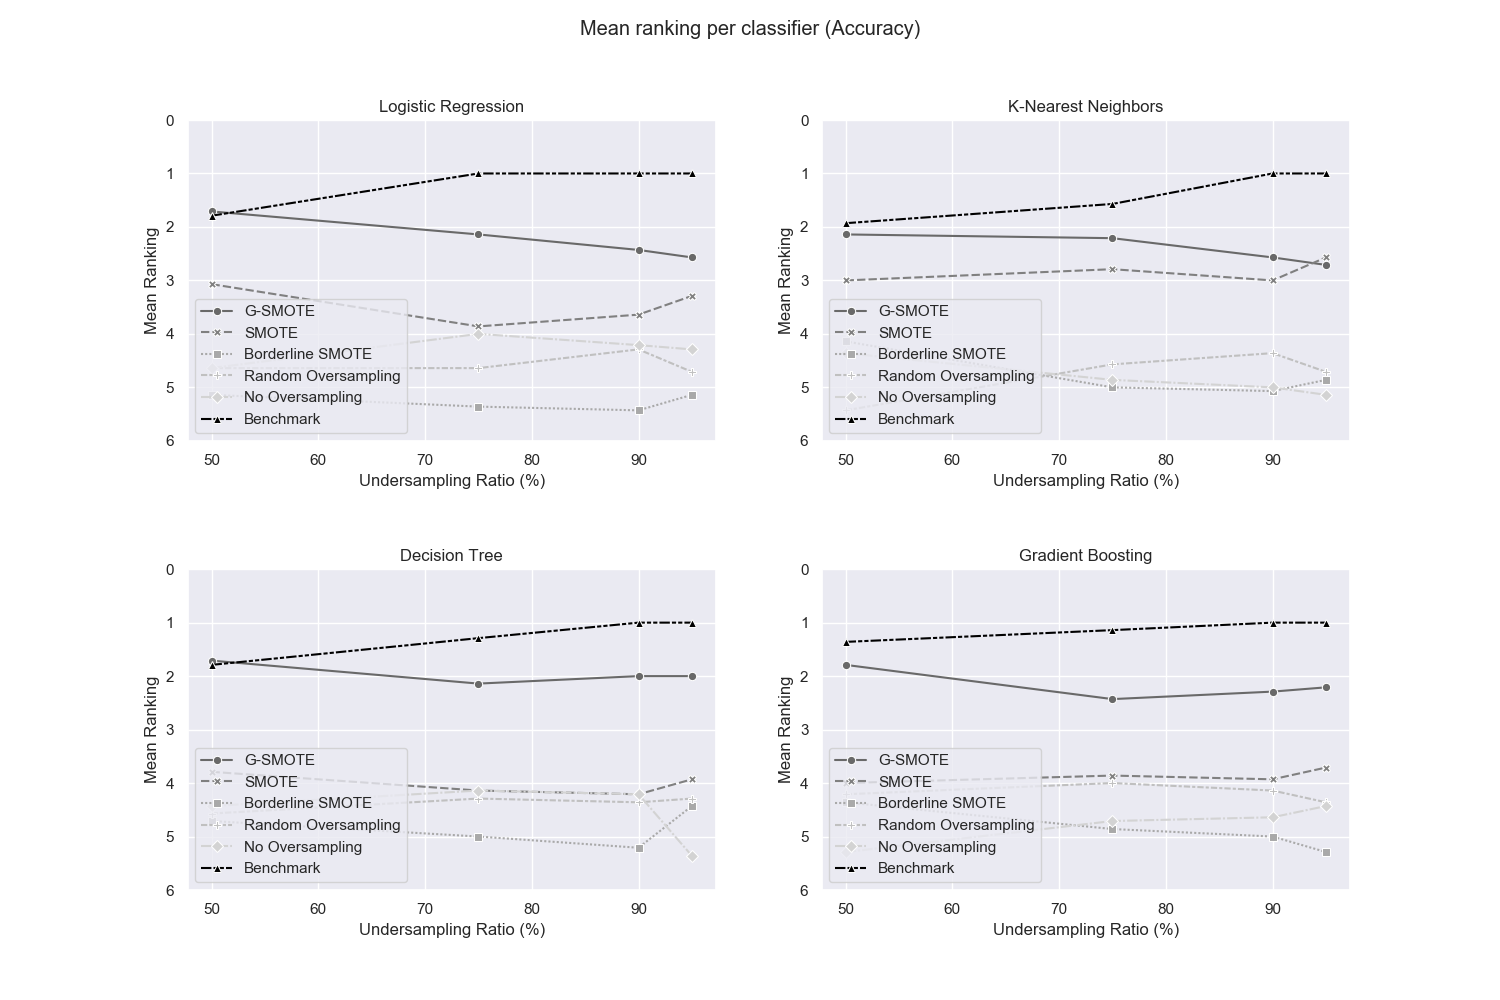
\includegraphics[width=1\linewidth]
		{../analysis/mean_ranking_per_classifier_accuracy}
	\caption{Mean ranking per classifier (Accuracy)}
	\label{fig:mean_ranking_per_classifier_accuracy}
\end{figure}

Looking at the graphs, G-SMOTE is ranked on the top place when comparing with
SMOTE, Borderline SMOTE, Random Oversampling and No Oversampling. Additionally,
G-SMOTE slightly outperforms the Benchmark method using the classifiers Logistic
Regression and Decision Tree in the mean ranking. 

\subsection{Statistical Analysis}

To confirm the significance of the above presented results we apply the Friedman
test as well as the Holm Test on the above results. The application of the
Friedman test is presented below:

\begin{center}
	\begin{footnotesize}
		\csvreader[
		longtable=llll,
		table head=
		\toprule\mdseries Classifier & \mdseries Metric & \mdseries p-value & 
		\mdseries Significance \\
		\midrule\endhead
		\bottomrule\endfoot,
		late after line=\\,
		before reading={\catcode`\#12},
		after reading={\catcode`\#12},
		]{../analysis/friedman_test.csv}
		{1=\classifier,2=\metric,3=\pvalue,4=\significance}
		{\classifier & \metric & \pvalue & \significance}
	\end{footnotesize}
	\addtocounter{table}{-1}
	\captionof{table}{Results for Friedman test}
	\label{tab:friedman_test.csv}
\end{center}

Therefore, the null hypothesis of the Friedman test is rejected at a 
significance level of a = 0.05, i.e. the over-samplers do not perform similarly 
in the mean rankings for any combination of classifier and evaluation metric.

The Holm's method is applied to adjust the $\text{p-values}$ of the paired 
difference test with G-SMOTE algorithm as the control method. The results are 
shown in table \ref{tab:holm_test}:

\begin{center}
	\begin{footnotesize}
		\csvreader[
		longtable=llllll,
		table head=
		\toprule\mdseries Classifier & \mdseries Metric & \mdseries NONE & 
		\mdseries RANDOM & \mdseries SMOTE & \mdseries B-SMOTE\\
		\midrule\endhead
		\bottomrule\endfoot,
		late after line=\\,
		before reading={\catcode`\#12},
		after reading={\catcode`\#12},
		]{../analysis/holms_test.csv}
		{1=\classifier,2=\metric,3=\none,4=\random,5=\smote,6=\bsmote}
		{\classifier & \metric & \none & \random & \smote & \bsmote}
	\end{footnotesize}
	\addtocounter{table}{-1}
	\captionof{table}{Adjusted $\text{p-values}$ using Holm test (B-SMOTE 
	corresponds to Borderline 
	SMOTE)}
	\label{tab:holm_test}
\end{center}

At a significance level of a = 0.05 the null hypothesis of the Holm's test is
rejected for 25 out 32 combinations. This indicates that the proposed method
outperforms all other methods in most cases.  

\section{Conclusions}

This paper illustrates an effective solution to mitigate the small dataset
problem in binary classification tasks. As shown above, the over-sampling
algorithm G-SMOTE has the ability to generate high quality artificial samples
and improve the prediction accuracy of various classifiers. This improvement
relates to its capability of increasing the diversity of new instances while
avoiding the generation of noisy samples. An important point is that G-SMOTE
significantly improves classification performance compared to the case where
only the small data are used. Also G-SMOTE outperforms standard over-sampling
approaches such Random Over-Sampling and SMOTE. Finally, G-SMOTE implementation
is available on (\url{https://github.com/AlgoWit/geometric-smote}).

\bibliography{references}
\bibliographystyle{apalike}

\end{document}
